% !TEX root = ../main.tex
%-------------------------------------------------------------------------------
%-------------------------------------------------------------------------------
\section{OSE Research}
%-------------------------------------------------------------------------------
%-------------------------------------------------------------------------------
\begin{frame}\frametitle{Eckstein--Keane--Wolpin models}



  	  \begin{multicols}{2}
  	    \heading{Understanding individual decisions}\vspace{0.3cm}
  	    \begin{itemize}\setlength\itemsep{1em}
          \item Human capital investment
          \item Consumption -- savings decision
  	    \end{itemize}

        \pause

  	    \heading{Predicting effects of policies}\vspace{0.3cm}
  	    \begin{itemize}\setlength\itemsep{1em}
          \item Welfare programs
          \item Tax schedules
  	  \end{itemize}
  	  \end{multicols}
\pause
\hspace{0.3cm}$\Rightarrow$ transdisciplinary research on their \alert<4>{economics}, \alert<5>{data}, and \alert<6>{computation}

\end{frame}
%-------------------------------------------------------------------------------
%-------------------------------------------------------------------------------
\begin{frame}\frametitle{Research projects}

\vspace{0.3cm}\heading{Economics and data}\vspace{0.3cm}

\begin{itemize}\setlength\itemsep{1em}
	\item \makebox[4cm][l]{\alert<1>{Biased expectations}}
                \only<1>{
                        \explanation{
                                Incorporate subjective expectations\\
                                Collaboration with DIW for SOEP-IS data collection
                        }
                }
	\item \makebox[4cm][l]{\alert<2>{Robust decisions}}
                \only<2>{
                        \explanation{
                                Account for ubiquitous uncertainties \\
                                Robust decision in light of model misspecification
                        }
                }
	\item \makebox[4cm][l]{\alert<3>{Vocational training}}
				\only<3>{
				        \explanation{%
				                Distinguish vocational and general education\\
				                Collaboration with IZA to study case of Germany
	                  }
                }
	\item \makebox[4cm][l]{\alert<4>{Option value}}
                \only<4>{
                        \explanation{%
                                Schooling reform for identification and validation\\
                                Collaboration with Statistics Norway
						}
                }

\end{itemize}
\end{frame}

%-------------------------------------------------------------------------------
%-------------------------------------------------------------------------------
\begin{frame}\frametitle{Research projects}

\vspace{0.3cm}\heading{Computation}\vspace{0.3cm}

\begin{itemize}\setlength\itemsep{1em}
  \item \makebox[4.5cm][l]{\alert<1>{Uncertainty quantification}}
                \only<1>{
                        \explanation{
                                Capture parametric uncertainty\\
                                Assess competing policy implications
                        }
                }
                \item \makebox[4.5cm][l]{\alert<2>{Global optimization}}
                \only<2>{
                        \explanation{%
                                Explore estimation uncertainty\\
                                Acknowledge multiplicity of local minima
                                  }
                }
  \item \makebox[4.5cm][l]{\alert<3>{HPC implementation}}
                        \only<3>{
                                \explanation{
                                Enable increased realism and auditing of economic models\\
                                Exploit large-scale parallelism on supercomputers
                                }
                        }
\end{itemize}
\end{frame}
%-------------------------------------------------------------------------------
%-------------------------------------------------------------------------------
\begin{frame}\frametitle{Community code}

\vspace{0.3cm}\textbf{\raisebox{-0.04cm}{
\includegraphics[height=0.60cm]{material/crop-respy-logo-bare.pdf}}\hspace{0.05cm} {\Large respy}}\vspace{0.50cm}

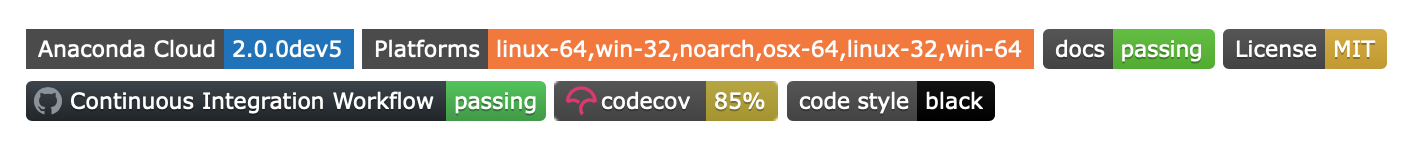
\includegraphics[width=0.9\textwidth]{material/crop-respy-engineering.png}\\\vspace{0.65cm}

A research code for the flexible specification, simulation, and estimation of Eckstein--Keane--Wolpin models.\\\vspace{0.65cm}

\textbf{Docs} \hspace{0.25cm} \href{https://respy.readthedocs.io/en/latest/}{\texttt{respy} Read the Docs}

\end{frame}
%-------------------------------------------------------------------------------
%-------------------------------------------------------------------------------
\begin{frame}\frametitle{Code as research}


  \begin{multicols}{2}
    \heading{Ecosystem}\vspace{0.3cm}
    \begin{itemize}\setlength\itemsep{1em}
      \item Permissive license
      \item Online documentation
      \item Benchmark data sets
      \item Retreat
    \end{itemize}

    \pause

    \heading{Infrastructure}\vspace{0.3cm}
    \begin{itemize}\setlength\itemsep{1em}
      \item Research software engineer
      \item Pre-doc position
      \item Lectures
      \item Courses
  \end{itemize}
  \end{multicols}

\end{frame}
%-------------------------------------------------------------------------------
%-------------------------------------------------------------------------------
